\section{Dataset}
In our work we employ the DEAM Dataset (\textit{MediaEval Database for Emotional Analysis in Music}) provided by the \textit{Swiss Center for Affective Sciences of the University of Geneva, Switzerland}.
The dataset consists of 2058 songs annotated with valence and arousal values both continuously (per-second) and over the whole song and csv files containing features extracted from every song.

In particular, our work is focused on the first 1802 songs, on the averaged annotations of the dataset and on the features extracted from the music database, both features already provided within the dataset and features extracted ex novo, and in order to avoid over-fitting, we split the dataset into training set and testing set using sklearn model\_selection library.


\subsection{Music database}

The music database consists of royalty-free music from several sources: \textit{freemusicarchive.org} (FMA), \textit{jamendo.com}, and the \textit{medleyDB dataset} \cite{bittner2014medleydb}. There are 1,744 clips of 45 seconds from FMA and 58 full length songs, half of which come from medleyDB and another half from Jamendo.\cite{aljanaki2017developing}
The provided 45 seconds excerpts have all been re-encoded to have the same sampling frequency (i.e, 44100Hz) and have been extracted from random (uniformly distributed) starting point in a given song. Both the 45 seconds clips and full songs are provided in MPEG layer 3 (MP3) format.\cite{soleymani2016deam}

The music from the FMA was in rock, pop, soul, blues, electronic, classical, hip-hop, international, experimental, folk, jazz, country and pop genres. The music from the MedleyDB dataset in addition had music in world and rap genres, and the music from Jamendo also had reggae music. For 2014 and 2015 data set, music have been manually checked and the files with bad recording quality or those containing speech or noise instead of music have been excluded. For each artist, have been selected no more than 5 songs to be included in the dataset. For medleyDB and Jamendo full-length songs, have been selected songs which had emotional variation in them, using an existing dynamic MER algorithm for filtering and manual final selection\cite{anna2015emotion}.


\subsection{Annotations}

The dataset from 2013 and 2014 contains annotations on 45 seconds excerpts extracted from random points in songs. Each excerpt was annotated by a minimum of 10 workers and the dynamic annotations were collected using a web-interface on a scale from -10 to 10, where workers could dynamically annotate the songs on valence and arousal dimensions separately while the song was being played.~\cite{aljanaki2017developing}

Then averaged annotations have been generated with 2Hz sampling rate and in addition to the average, the standard deviation of the annotations is provided.~\cite{soleymani2016deam}


\subsection{Features}

A set of features extracted by \emph{openSMILE}~\cite{opensmile} for 500ms windows is provided with the dataset and a set of different features is extracted from the 45 seconds song excerpts using \emph{Librosa}~\cite{librosa} and computing 5 different statistical moments (mean, standard deviation, maximum, minimum and kurtosis).

We make several attempts in order to achieve best results in the cross-validation step \hyperref[sec:evaluation]{(see Evaluation section)} so we try separating tracks in two sets, a "high-annotation" set and a "low-annotation" set, both for valence and arousal mean values, and then plotting the distribution of values of a selected feature for the songs of each set. (e.g. see figure ~\ref{fig:va_mean-spectral_flatness-dists})

\begin{figure}
	\centering
	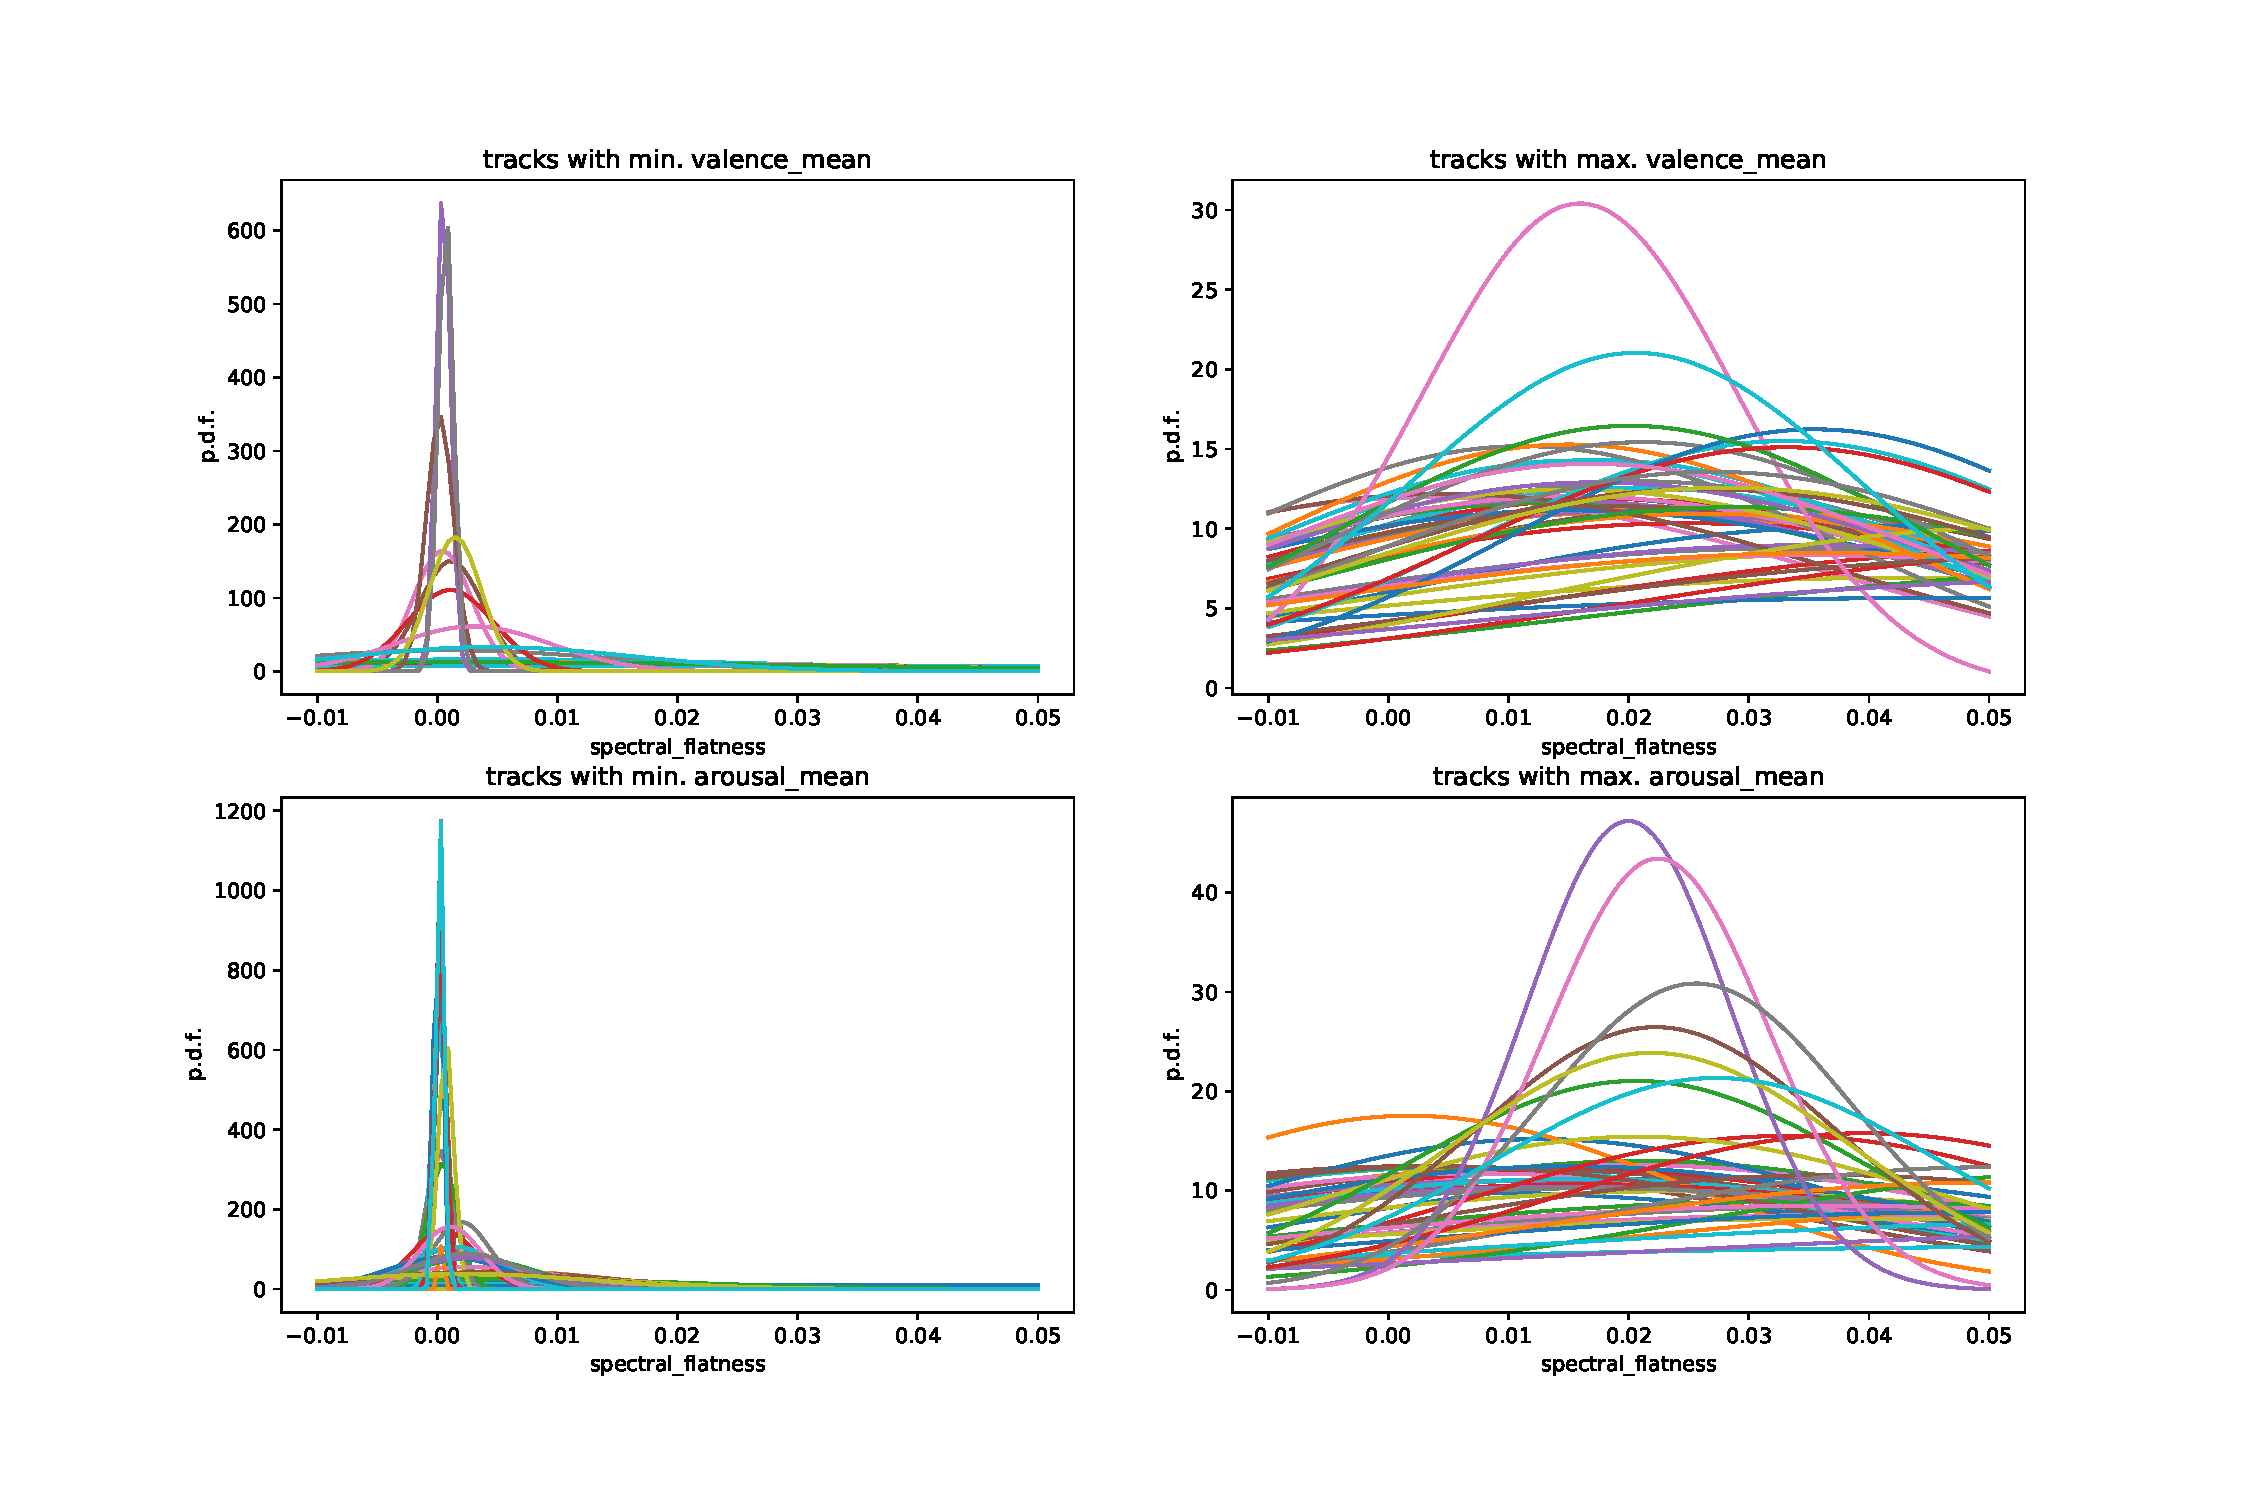
\includegraphics[width=0.9\linewidth]{assets/va_mean-spectral_flatness-dists.pdf}
	\caption{Spectral flatness distribution}
	\label{fig:va_mean-spectral_flatness-dists}
\end{figure}

Then we realize that a better way to visualize features might be to plot feature-vs-annotation scatters (e.g. see figure ~\ref{fig:scatter-spectral_bandwidth_amean}) and we notice several linear relationships between a feature and valence and/or arousal values. Therefore we use these results to make a preliminary manual feature selection through a Pipeline. In particular we select different features depending on the annotation to be predicted and discard unneeded features.

\begin{figure}
	\centering
	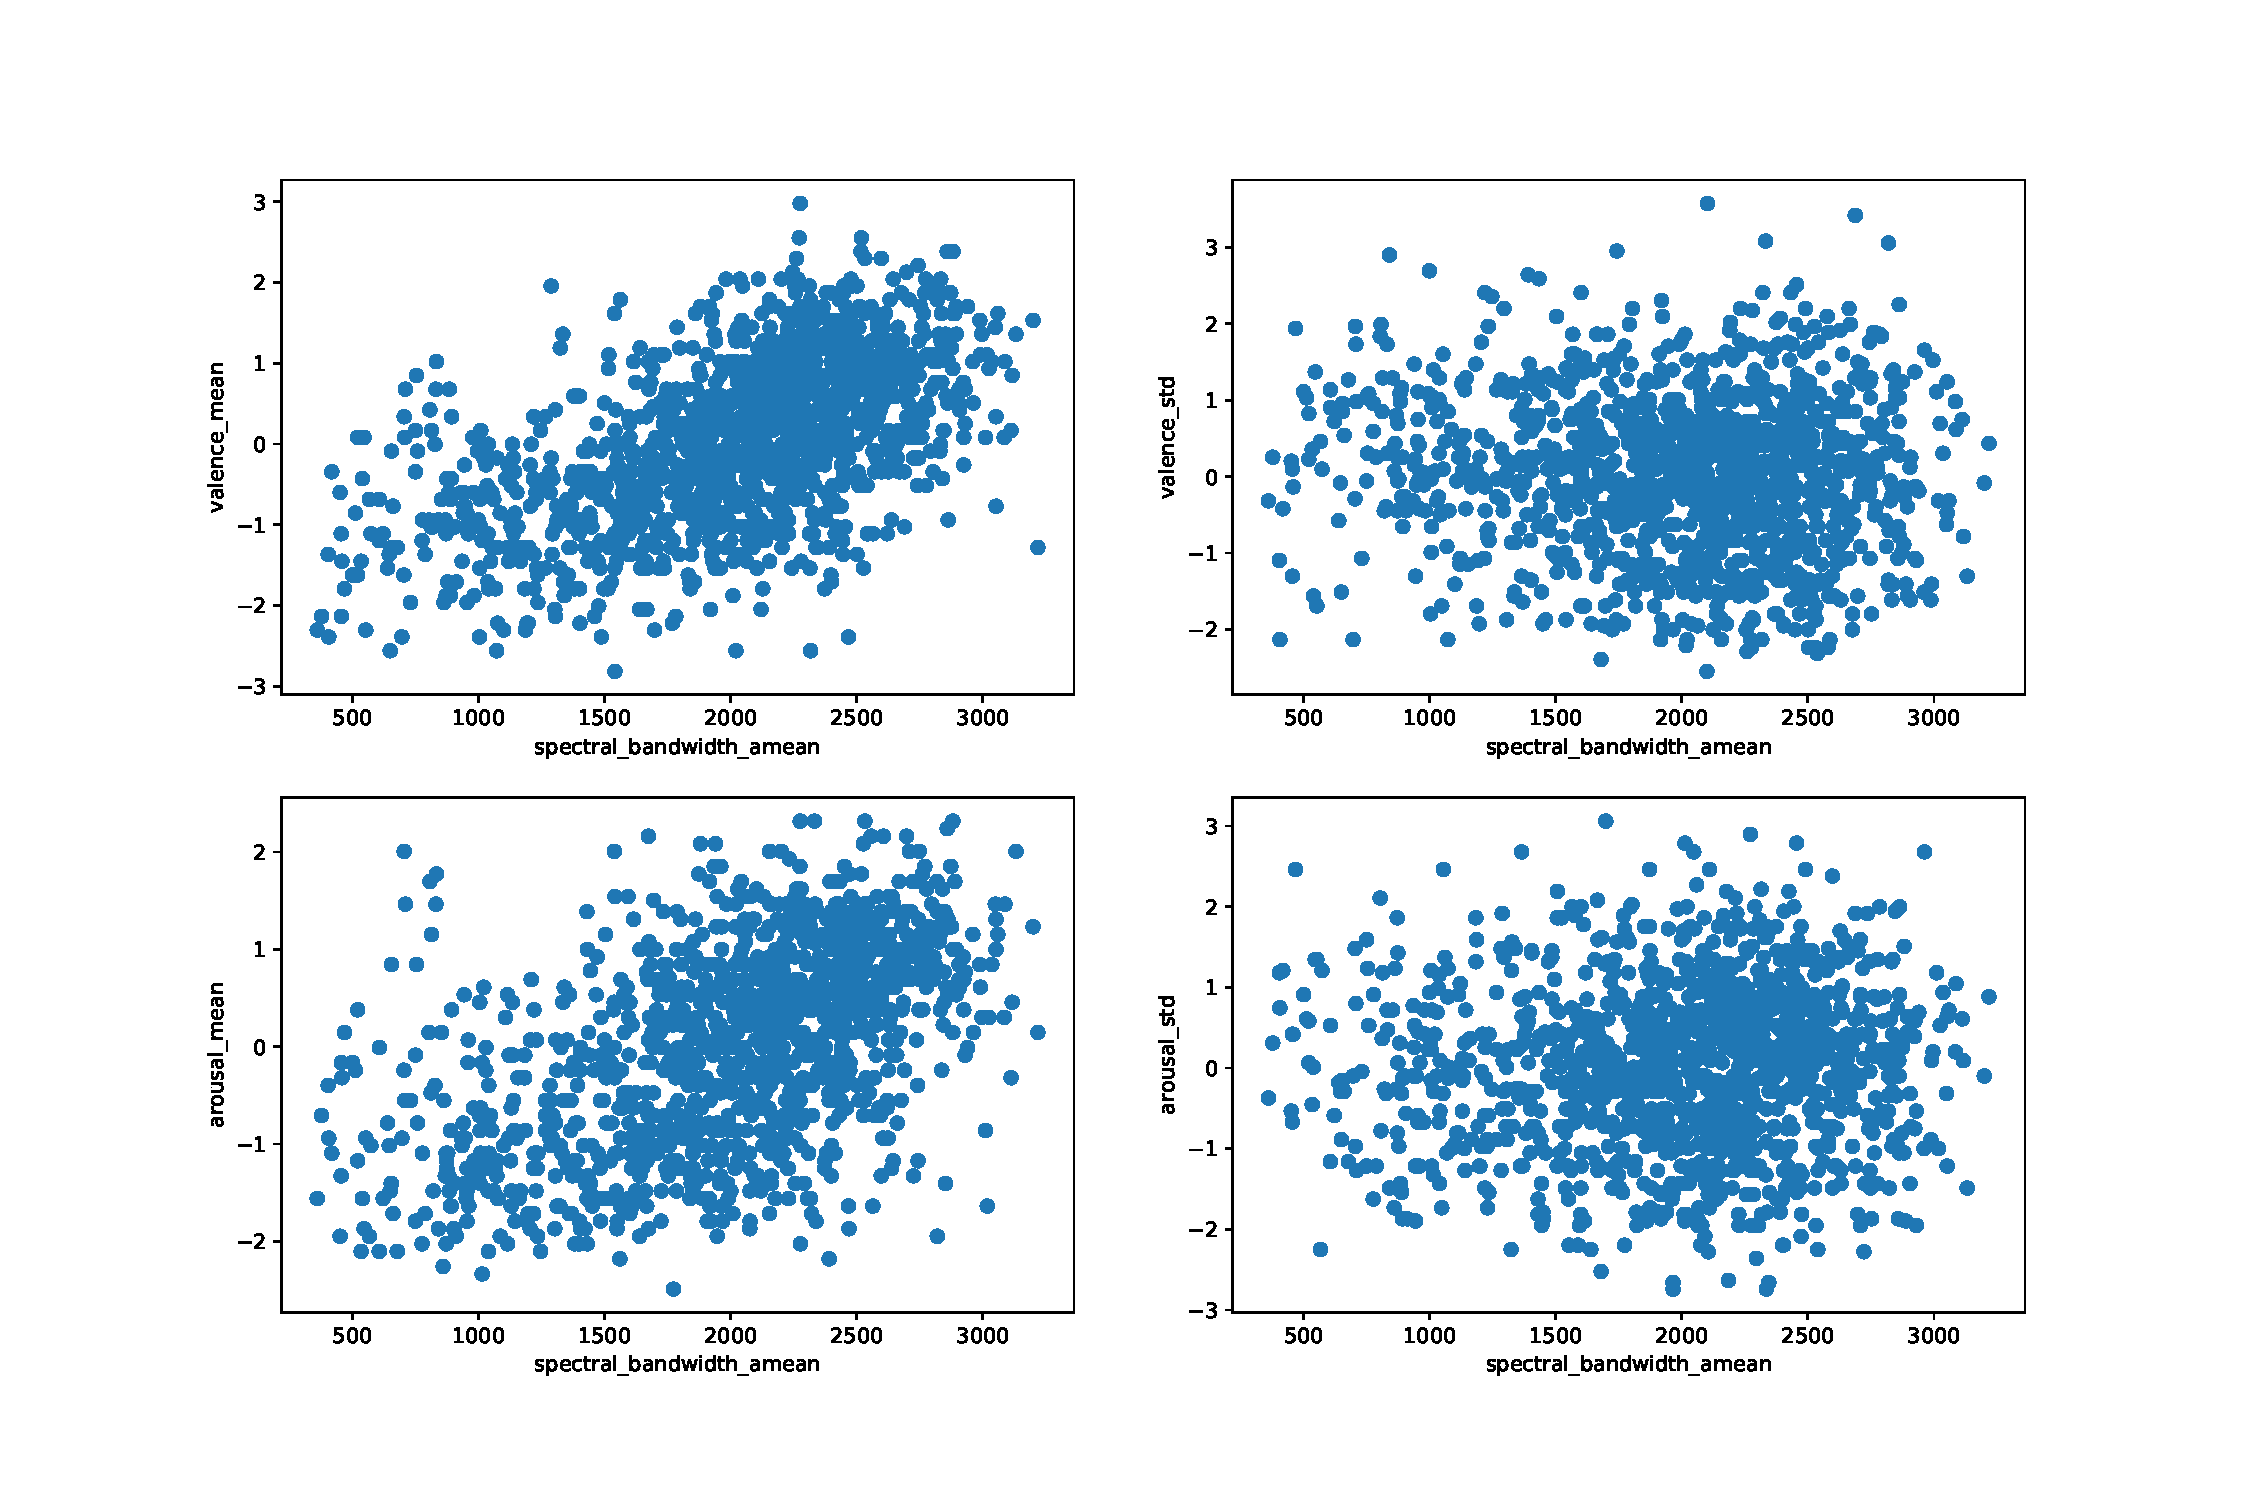
\includegraphics[width=0.9\linewidth]{assets/scatter-spectral_bandwidth_amean.pdf}
	\caption{Spectral Bandwidth vs. Annotations scatter plot}
	\label{fig:scatter-spectral_bandwidth_amean}
\end{figure}

Finally, in addition to manual selection, we filter out unneeded or redundant features using automatic feature selection tools.